%% Load document class fithesis2
%% {10pt, 11pt, 12pt}
%% {draft, final}
%% {oneside, twoside}
%% {onecolumn, twocolumn}
\documentclass[12pt,final,oneside]{fithesis2}

%% Basic packages
\usepackage[english]{babel}
\usepackage{cmap}
\usepackage[T1]{fontenc}
\usepackage{lmodern}
\usepackage[utf8]{inputenc}
\usepackage{graphicx}


%% Additional packages for colors, advanced
%% formatting options, etc.
\usepackage{color}
\usepackage{microtype}
\usepackage{url}
\usepackage{cslatexquotes}
\usepackage{fancyvrb}
\usepackage[small,bf]{caption}
\usepackage[plainpages=false,pdfpagelabels,unicode]{hyperref}
\usepackage[all]{hypcap}

%% Fix long URLs in DVIs
\usepackage{ifpdf}

%% Source code highlight

\usepackage{floatrow}
\usepackage[chapter]{minted}
\usemintedstyle{trac}
%get caption above code
\floatsetup[listing]{style=Plaintop}
%caption style    
%\captionsetup[listing]{format=listing, singlelinecheck=false, margin=pt, font={bf}}
%\captionsetup[listing]{format=listing}
%fancyvrb frame
\renewcommand{\listingscaption}{Example}


\DeclareGraphicsExtensions{.pdf,.png,.jpg}

\ifpdf
\else
  \usepackage{breakurl}
\fi

%% Packages used to generate various lists
\usepackage{makeidx}
\makeindex

\usepackage[xindy]{glossaries}
\makeglossary

%% Use STAR and CIRCLE signs for nested
%% itemized lists
\renewcommand{\labelitemii}{$\star$}
\renewcommand{\labelitemiii}{$\circ$}

%% Title page information
\thesistitle{RESTEasy integration with Apache Camel project}
\thesissubtitle{Master's thesis}
\thesisstudent{Roman Jakubčo}
\thesiswoman{false} %% Important when using Slovak or Czech lang
\thesisfaculty{fi}  %% {fi, eco, law, sci, fsps, phil, ped, med, fss}
\thesislang{en}     %% {en, sk, cs}
\thesisyear{Spring 2015}
\thesisadvisor{Mgr. Marek Grác, PhD.}

%% Beginning of the document
\begin{document}

%% Front page with a logo and basic thesis information
\FrontMatter
\ThesisTitlePage

%% Thesis declaration (required)
\begin{ThesisDeclaration}
  \DeclarationText
  \AdvisorName
\end{ThesisDeclaration}

%% Thanks (optional)
\begin{ThesisThanks}
 
\end{ThesisThanks}

%% Abstract (required)
\begin{ThesisAbstract}

\end{ThesisAbstract}

%% Keywords (required)
\begin{ThesisKeyWords}

\end{ThesisKeyWords}

%% Beginning of the thesis itself
\MainMatter

%% TOC (required)
\tableofcontents

%% Thesis text structured using
%% chapters, sections, subsections, etc.
\chapter{Introduction}


\chapter{Technologies}
This chapter describes technologies that are used for implementation of Camel RESTEasy  component. Each subsection introduces the technology and tries to explain what is its main functionality and common usage.

\section{Apache Camel}
Apache Camel is a open source rule-based routing and mediation framework implemented in Java. It is based on theory of Enterprise Integration Patterns or EIP, described in the book with same name written by Gregor Hohpe and Bobby Wolf\cite{eip}.

Its main focus is on integration and interaction between various applications or systems for which Camel can provide standalone routing, transformation, monitoring and many other things. From this point of view Camel may seems like ESB\footnote{ESB - Enterprise Service Bus}, but this is not the case, because Camel doesn't provide a container support or reliable message bus, but it can be deployed into one and create full integration platforms(also know as ESB) like Apache ServiceMix\footnote{\url{http://servicemix.apache.org/}}, JBoss Fuse\footnote{\url{http://www.jboss.org/products/fuse/overview/}} and JBoss Fuse Service Works. 

Camel also has extensible and modular architecture that allows implementation and seamlessly plug in support for new protocols and this architectural design makes Camel lightweight, fast and easy extendable for developers.\cite{camel-in-action}

\subsection{The core principles/features of Camel}
Camel is using convention over configuration approach to describe given task by domain-specific language (DSL) in declarative way. This way Camel minimize number of lines of the source code that is needed for implementation of integration scenarios. Another key feature that helps with this task is usage of theory of EIPs, which are already integrated in DSL and also getting the most from their potential. 

Another fundamental principle of Camel is that it makes no assumptions about the data format. This feature is important because it makes possible for developers to integrate  systems together without any need to convert data to some canonical format. This way there are no limitations for integration of any kind of systems together\cite{camel-in-action}.

\subsection*{Routing and mediation engine}
One of the core features of Camel is its routing and mediation engine. A routing engine selectively moves a data from one destination to another based on the route’s configuration. Users also can define their own rules for routing, add processors to modify the data, filter them based on some predicate and at the end decide the final destination for the delivery.

\subsection*{Enterprise integration patterns}
Like it is mentioned before Camel is based primarily on EIPs. EIPs describe integration problems and their solutions and also provide some basic vocabulary but the problem is this vocabulary isn't formalized. And into this comes Camel with its language which describes the integration solutions and tries to formalized the vocabulary. There's almost a one-to-one relationship between the patterns described in
Enterprise Integration Patterns and the Camel DSL\footnote{\url{http://camel.apache.org/enterprise-integration-patterns.html}}.
Almost all of the EIPs that are defined in the book are implemented as Processors or sets of Processors in the Camel. Processors are used for manipulation of messages between destinations specified in the Camel route.\cite{camel-dzone}



\subsection*{Domain-specific language}
There are few other integration frameworks with DSL and also some have support for describing route rules in XML, but bonus that comes with Camel is its the support for specifying DSLs in regular programming languages as Java, Groovy, Ruby and even Scala. Of course there is also possibility to describe the route in XML document. 

\begin{listing}[ht]
	\inputminted[]{java}{sources/java_dsl_example.java}
	\caption{Java DSL definition of route}

\end{listing}

\begin{listing}[ht]
	\inputminted[]{xml}{sources/xml_example.xml}
	\caption{XML definition of route }

\end{listing}

\begin{listing}[ht, p!]
	\inputminted[]{java}{sources/scala_example.java}
	\caption{Scala definition of route }

\end{listing}


\subsection*{Modular and pluggable architecture}
The next feature is the approach to the architecture, which is done in modular way. This means, that Camel can be easily extended to consume data from endpoint and produce data to endpoint. Camel is describing this as developing a new component, where each component is responsible for consuming or producing data for some specific endpoint and technology e.g. file, HTTP and many others. When developers want to develop a new component for some unique system and add its functionality to the Camel, they just need to follow structure specified by the framework and extend core classes. 

By default Camel ships with the few most basic components called camel-core. This bundle includes 24 components including components like bean, file, log, seda and mock. Plus there are many more components developed by the Apache community and also third-parties\footnote{\url{http://camel.apache.org/components.html}}. There are already developed components that can be used for the most common integration scenarios that occur in systems. Some components worthy of note are web services including SOAP\footnote{SOAP} or REST\footnote{REST}, JMS\footnote{JMS}, specialized JMS component for Apache ActiveMQ\footnote{\url{http://camel.apache.org/activemq.html}} or components for different database connections.


\subsection*{Configuration}
As mentioned before Camel uses convention over configuration paradigm to minimize configuration requirements so that developers don't need to learn complicated configuration options and focus on more important things.  This is reflected on configuration of endpoints in route definitions with URI options as can be seen on example \ref{uri-option}.
\begin{listing}[ht]
	\inputminted[]{java}{sources/uri.java}
	\caption{URI options configurations}
	\label{uri-option}
\end{listing}

\subsection*{Type converters}
Another feature of Camel which is one of the top features for Camel Community and that are build-in automatic converters. Out of the box Camel ships with more than hundred and fifty converters\cite{camel-in-action}. Plus if there is no converter for your types, there is possibility to create new custom converters for your specific types. Usage of the converter can be seen on example \ref{converter} and the example also demonstrates how is the converter used by Camel without user's knowledge in \textit{getBody} method and its parameter.

\begin{listing}[ht, p!]
	\inputminted[]{java}{sources/converter.java}
	\caption{TypeConverter invocation}
	\label{converter}
\end{listing}


\subsection*{Lightweight framework}
From the start the whole framework was designed to be undemanding and lightweight as possible. The core library has only about 1.6 MB and third parties dependencies are kept at minimum. This way Camel can be easily embedded into any platform, which can be e.g. OSGi\footnote{OSGi} bundle, Spring application, Java EE application or web application. 

\subsection{Message model}
Until now we talk about sending data from one endpoint to another. That is exactly what is Camel doing but in reality it is sending and receiving messages which encapsulate the data. There two abstractions classes that are use for modelling messages in Camel and these are:
\begin{itemize}
\item
\texttt{org.apache.camel.Message} -- the basic entity containing data that is routed in the Camel 

\item
\texttt{org.apache.camel.Exchange} -- special abstraction used in Camel for exchange of messages, that has \textit{in} message and \textit{out} message as a reply

\end{itemize} 

\subsection*{Message}
Message object is representing data that is used by systems to communicate with each other. Messages are sent in one direction from a sender to a receiver. The message object consists of body, headers and optional attachments. All messages must be uniquely identified with an unique identifier(UID). The format of UID is not guaranteed and it is dependent on the used protocol. If the protocol doesn't have UID scheme, then generic generator from the framework is used.

Headers are name-value pairs associated with the message, similar to HTTP protocol. They provide additional information about the message such as sender identifiers, encoding, content type or authentication parameters. They are stored in a map within the message and each name of the header is unique case insensitive string and the value can be any Java object.

Body is representing content of the message and its type is generic Java Object, so message can store any kind or type of content. The sender should send body type acceptable by the receiver. If this is not the case then manual transformation inside the route is needed or more conveniently type converters are automatically used by the Camel.


\subsection*{Exchange}
An \textit{Exchange} is defined as message's container encapsulating the \textit{Message} used during routing. There are various types of interactions between systems and they are supported by the \textit{Exchange}. These interactions are called message exchange patterns (MEPs) and they are used to specify messaging styles in the property of the  \textit{Exchange}. This property has to two different messaging styles where one is one-way and the other one is request-response. 

The request-response or \textit{InOut} called in the Camel, is probably the more well-known style because it is used in HTTP-based transport, where client requests to retrieve a web page and it is waiting for the reply from the server. One-way is defined as \textit{InOnly} and for example is primarily use in JMS, where message is sent to the queue and sender doesn't need any response from the queue. These two types are just the basic ones, but Camel provides few more special cases\footnote{Exchange patterns in Camel\url{
http://camel.apache.org/maven/current/camel-core/apidocs/org/apache/camel/ExchangePattern.html}}.\cite{camel-exchange}

The \textit{Exchange} is little bit more complex than the \textit{Message} and it is consisting from\cite{camel-in-action}:
\begin{itemize}
\item
Exchange ID -- is unique ID that identifies the exchange and it is also automatically generated by the Camel if ID is not explicitly set.

\item
MEP -- defines type of messaging style.

\item
Exception -- If an error occurred during routing, then \textit{Exception} is set into this field.

\item
Properties -- various properties of the \textit{Exchange} used by Camel, similar to headers in \textit{Message}, but with difference that the properties last for the duration of entire exchange and contain global information, whereas message header are specific to the \textit{Message}. They can be also edited by developers.

\item
In message -- mandatory input message containing request message.

\item
Out message -- optional message containing reply message if the MEP is set to \textit{InOut}.
\end{itemize}


\subsection{Camel's architecture}
This chapter will describe architecture of the Camel from high-level and then take closer look on some specific concepts. The basic architecture of the Camel is shown in the figure \ref{camelContext} and should help with understanding of the runtime of \textit{CamelContext}.

\begin{figure}[!h]
\centering
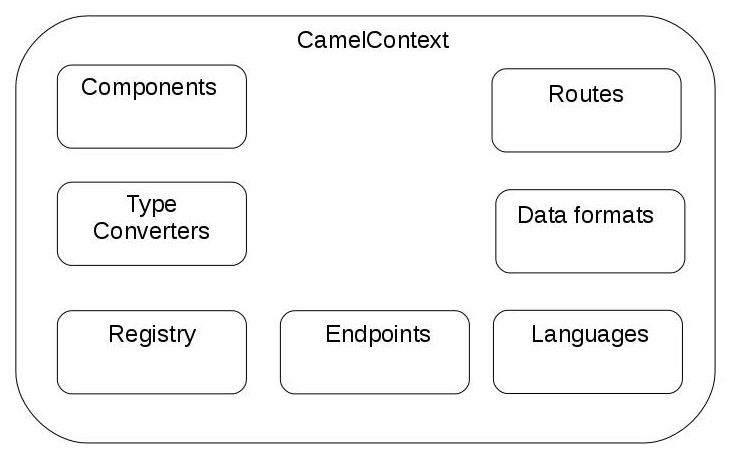
\includegraphics[width=0.9\linewidth]{sources/CamelContextCrop.jpg}
\caption{Overview of CamelContext}
\label{camelContext}
\end{figure}

\subsection*{Camel context}
From the figure \ref{camelContext} it is clear that CamelContext is somewhat similar to container but more precisely it is Camel's runtime system. This system keeps everything together and provides services during the runtime that are:
\begin{itemize}
\item
Routes -- routes that have been added to the context

\item
Endpoints --endpoints that have been created in context

\item
Components -- components used by the application and they can be added on the fly

\item
Type converters -- loaded type converters by the context

\item
Data formats -- data formats loaded into to the context

\item
Languages -- Camel supports different languages used in the expressions and these are loaded into the context

\item
Registry -- registry is used for the look up of beans. JNDI\footnote{JNDI} registry is used by default, but if Camel is deployed into Spring or OSGi container then it uses native registry mechanism specific to these technologies.

\end{itemize}

\subsection*{Routing engine and routes}
The routing engine is the thing that actually moves messages, but is not visible to users. It guarantees correct routing from the sender to the receiver.

Routing engine is using routes for its routing. Routes are the essence of the Camel and are the main and only approach how to specify what should be moved where for the routing engine. This means that the route must hold definition of input source to output target. There many possibilities for definition of the route, but the simplest way is to define route as a chain of processors\cite{camel-in-action}. Similar to Message or Exchange, each route has unique identifier that is used for different operation inside of Camel like monitoring, starting or stopping the route. One of the constraint for the route is restriction for the number of input sources, where each route must have exactly one input source that is tied to input endpoint and there can be one or several output targets.

\subsection*{Processors}
As mentioned before the simplest route consists from the chain of processors. The processor represents a node responsible for using, creating or modifying content of incoming \textit{Exchange} and also its headers. In the chain of processors, exchanges moves during routing from one processor to a another, in the their order defined in the route. This way a route can be seen as graph with nodes where output from the one node is input of another.

As stated previously, almost all built-in processors or their combinations are implementation of EIPs, but Camel also supports implementation of own custom processors and their easy addition to the route.

\subsection*{Component}
A components help with modular approach and they are main extension point in Camel. Their main purpose and task is to be a factory of endpoints. As mentioned before developers can create their new components, more information and detail on this topic will be given in subchapter \ref{component-devel}. 

\subsection*{Endpoint}
 
\section{Development of the new Camel component}\label{component-devel}

%\section{Integration}
%\section{REST architecture}
%\section{JBoss RESTEasy}
%\subsection{RESTful webservice}
%\subsection{JAX-RS 1.0}
%\subsection{JAX-RS 2.0}
%
%\chapter{Analysis and Design}
%\section{Requirements}
%\subsection{Camel consumer}
%\subsection{Camel producer}
%\section{Diagrams}
%\subsection{Data flow diagram}
%\subsection{Class diagram}
%\section{Design restrictions}
%
%\chapter{Implementation}
%\section{ssss}
%
%\chapter{Conclusion}






%% Lists of tables and figures, glossary, etc.
%%\printindex
%%\printglossary
%%\listoffigures
%%\listoftables

\begingroup
\def\tmpchapter{0}
\renewcommand{\chaptername}{}
\renewcommand{\thechapter}{}
%%\addtocontents{toc}{\setcounter{tocdepth}{-1}}
\chapter{References}
\renewcommand{\chapter}[2]{}% for other classes

\bibliographystyle{plain}
\bibliography{references}

\begin{thebibliography}{}
\bibitem{eip} HOHPE, Gregor and WOLF, Bobby. \textit{Enterprise integration patterns}. Boston: Addison-Wesley, c2003, li, ISBN 978-0321200686.
\bibitem{camel-in-action} IBSEN, Claus and ANSTEY,Jonathan. \textit{Camel in Action}. Greenwich, Conn.: Manning, c2011, xxxi, ISBN 19-351-8236-6.
\bibitem{camel-dzone} http://java.dzone.com/articles/open-source-integration-apache
\bibitem{camel-exchange} http://camel.apache.org/exchange-pattern.html

\bibitem{camel-web} APACHE. \textit{Apache Camel} [online]. 2004- [cite 2014-12-12]. Available at: \url{http://camel.apache.org/}

\bibitem{java-web} ORACLE. \textit{Java} [online]. \copyright{} 2004- [cite 2014-12-12]. Available at: \url{http://www.java.com/}			

%
\bibitem{camel-cookbook} CRANTON, Scott and KORAB, Jakub. \textit{Apache Camel Developer's Cookbook}.  Birmingham: Packt publishing, c2013, ISBN 9781782170303.
%
%\bibitem{dzone} DZONE RESEARCH. \textit{Guide to Enterprise Integration} [online]. 2014- [cite 2014-12-14]. Available at: \url{http://www.dzone.com/research/guide-to-enterprise-integration}
%
%%\bibitem{esb} THOMAS, Anne. \texit{https://www.gartner.com/doc/1405237/enterprise-service-bus-definition} [online]. 2007 - [cite 2014-12-14]. Available at: \url{https://www.gartner.com/doc/1405237/enterprise-service-bus-definition}




\end{thebibliography}

\endgroup
%% Additional materials
\appendix

\chapter{Appendix}


%% End of the whole document
\end{document}